\documentclass[a4paper,12pt]{article}
\usepackage{cmap}
\usepackage[utf8]{inputenc}
\usepackage[english, russian]{babel}
\usepackage[left=2cm,right=1cm,top=2cm,bottom=2cm]{geometry}
\usepackage[pdftex]{graphicx}
\usepackage{hyperref}
\usepackage{wrapfig}
\graphicspath{{img/}}
\usepackage{float}

\begin{document}

\thispagestyle{empty}

\begin{figure}[h]
	\centering
	
\includegraphics[scale=0.60]{title.png}
\end{figure}
\clearpage

\tableofcontents 
\clearpage

\section{Сокращения}

ПКМ - правая кнопка мыши.
\clearpage

\section{Кратко о SVN}
\setcounter{figure}{0}
\href{http://www.subversion.apache.org/}{SVN} - это система контроля версий,
которая зависит от центрального репозитория. Создана чтобы заменить систему
\href{http://www.nongnu.org/cvs/}{CVS}.

\subsection{Недостатки}

К недостаткам следует отнести постоянную необходимость ``находиться на
связи'' с репозиторием. Так, если репозиторий недоступен, Вы не сможете
зафиксировать изменения.

\subsection{Достоинства}

\begin{itemize}
\item
  Простота в освоении
\item
  Распространённость
\item
  Наличие
  \href{http://svnbook.red-bean.com/nightly/ru/svn-book.html}{русскоязычного
  руководства}, хоть и устаревшего (текущая версия SVN - 1.7, в
  руководстве описана версия 1.4) 
\end{itemize}
\clearpage
\subsection{Основы работы}

Для того чтобы хорошо ознакомиться с SVN, лучше для начала поработать с
консольным клиентом SVN (command line client).

\subsubsection{Установка}

\paragraph{Пользователям Windows}

Для установки консольного клиента необходимо скачать
\href{http://www.sliksvn.com/en/download}{дистрибутив} и установить в
любую директорию (\texttt{\%INSTALLATION\_PATH\%}). Ниже описан процесс
установки.

\begin{figure}[!h]
	\centering
	
\includegraphics[scale=0.90]{slik-svn-instalation-step-1.png}
	\vspace{-10pt}
	\caption{Установка консольного клиента, шаг 1}
\end{figure}

\begin{figure}[!h]
	\centering
	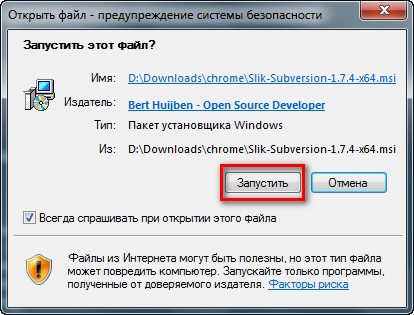
\includegraphics[scale=0.80]{slik-svn-instalation-step-2.png}
	\vspace{-10pt}
	\caption{Установка консольного клиента, шаг 2}
\end{figure}

\begin{figure}[h!]
	\begin{minipage}[h]{0.49\linewidth}
		\center{
			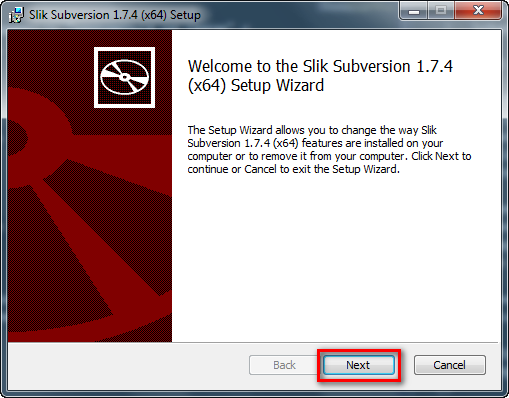
\includegraphics[scale=0.65]{slik-svn-instalation-step-3.png}
			\vspace{-10pt}
			\caption{Установка консольного клиента, шаг 3}
		}
	\end{minipage}
	\hfill
	\begin{minipage}[h]{0.49\linewidth}
		\center{
			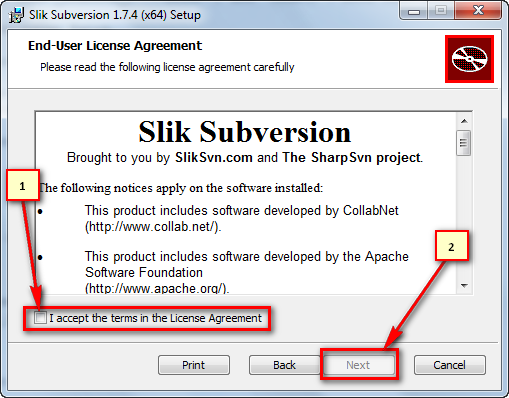
\includegraphics[scale=0.65]{slik-svn-instalation-step-4.png}
			\vspace{-10pt}
			\caption{Установка консольного клиента, шаг 4}
		}
	\end{minipage}
\end{figure}

Перед продолжением установки, запомните путь к директории, в которую
будет устанавливаться command line subsersion client.

\begin{figure}[h!]
	\begin{minipage}[h]{0.49\linewidth}
		\center{
			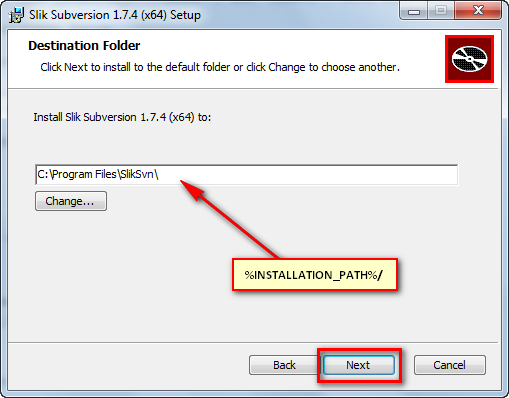
\includegraphics[scale=0.60]{slik-svn-instalation-step-5.png}
			\caption{Установка консольного клиента, шаг 5}
		}
	\end{minipage}
	\hfill
	\begin{minipage}[h]{0.49\linewidth}
		\center{
			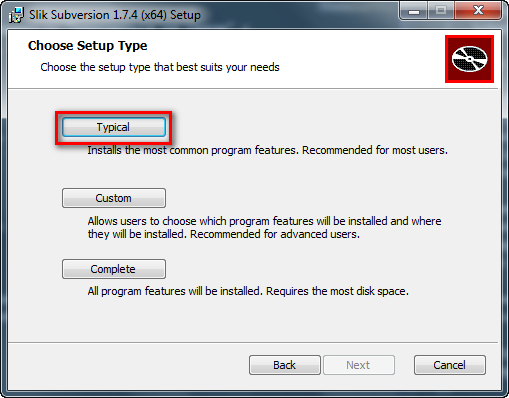
\includegraphics[scale=0.60]{slik-svn-instalation-step-6.png}
			\caption{Установка консольного клиента, шаг 6}
		}
	\end{minipage}
	\vfill
		\begin{minipage}[h]{0.49\linewidth}
		\center{
			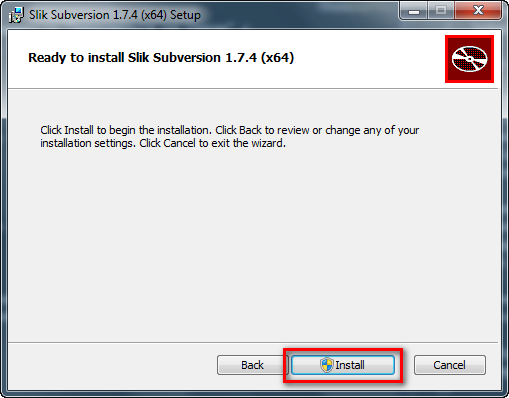
\includegraphics[scale=0.60]{slik-svn-instalation-step-7.png}
			\caption{Установка консольного клиента, шаг 7}
		}
	\end{minipage}
	\hfill
	\begin{minipage}[h]{0.49\linewidth}
		\center{
			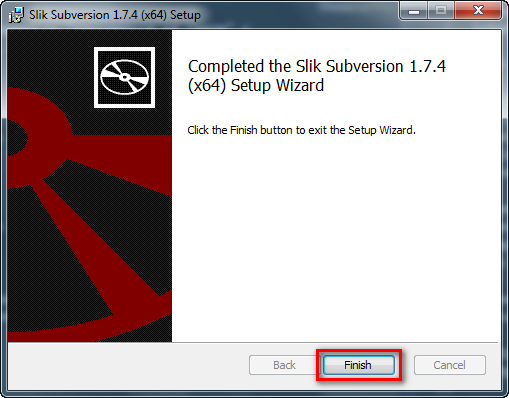
\includegraphics[scale=0.60]{slik-svn-instalation-step-8.png}
			\caption{Установка консольного клиента, шаг 8}
		}
	\end{minipage}
\end{figure}

Установка консольного клиента Subversion завершена. Теперь Вы можете
полноценно работать с этой системой контроля версий.

Для проверки работы консольного клиента запустите Командную строку
(cmd.exe) и выполните команду \texttt{svn help}. Эта команда выведет на
консоль все поддерживаемые команды консольного клиента. 

Если возникла ошибка и команды не вывелись необходимо добавить путь к бинарным
файлам в переменнуюю окружения \texttt{Path}.

Это можно сделать следующим образом:

\begin{figure}[h!]
	\begin{minipage}[h]{0.49\linewidth}
		\center{
			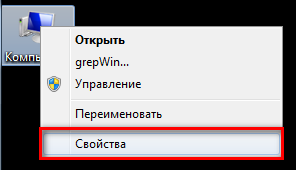
\includegraphics[scale=0.80]{slik-svn-configuration-step-1.png}
			\caption{Настройка переменной окружения \texttt{Path}, шаг 1}
		}
	\end{minipage}
	\hfill
	\begin{minipage}[h]{0.49\linewidth}
		\center{
			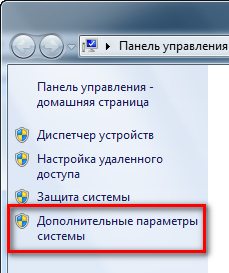
\includegraphics[scale=0.50]{slik-svn-configuration-step-2.png}
			\caption{Настройка переменной окружения \texttt{Path}, шаг 2}
		}
	\end{minipage}
\end{figure}
  
 \begin{figure}[h!]
	\begin{minipage}[h]{0.49\linewidth}
		\center{
			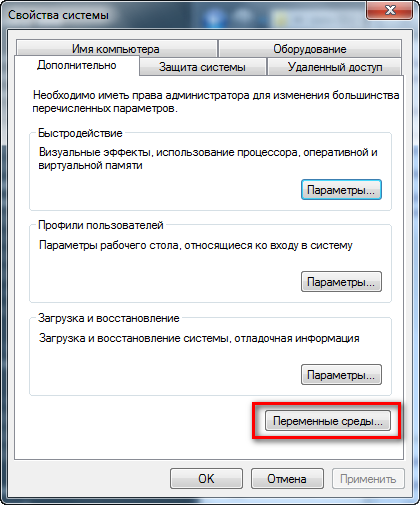
\includegraphics[scale=0.60]{slik-svn-configuration-step-3.png}
			\caption{Настройка переменной окружения \texttt{Path}, шаг 3}
		} 
	\end{minipage}
	\hfill
	\begin{minipage}[h]{0.49\linewidth}
		\center{
			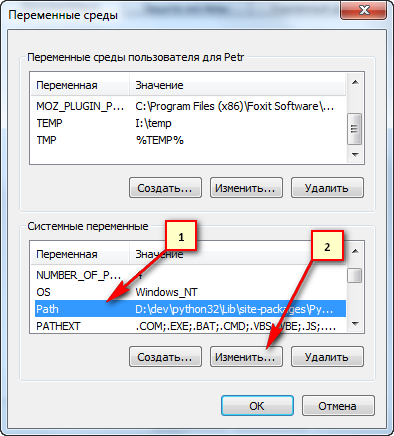
\includegraphics[scale=0.70]{slik-svn-configuration-step-4.png}
			\caption{Настройка переменной окружения \texttt{Path}, шаг 4}
		}
	\end{minipage}
\end{figure}

\begin{figure}[!h]
	\centering
	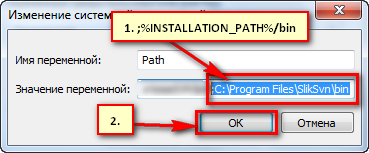
\includegraphics[scale=0.70]{slik-svn-configuration-step-5.png}
	\caption{Настройка переменной окружения \texttt{Path}, шаг 5}
\end{figure}

\paragraph{Пользователям Linux}
Для работы с SVN в Linux достаточно установить пакет Subversion.
Пример установки данного пакета для Ubuntu: \texttt{sudo apt-get install
subversion}
 
\subsubsection{Термины}

\begin{itemize}
\item
  \emph{Репозиторий} - это центральное хранилище данных. Используется
  для хранением файлов, директорий, которые были помещениы под контроль
  версий, и их ревизий.
\item
  \emph{Рабочая копия (working copy)} содержит файлы, директории и
  мета-данные, размещенные в служебном каталоге (директория
  \texttt{.svn}). В рабочей копии можно создавать, читать, изменять и
  удалять файлы. После фиксации все изменения попадут в репозиторий и
  будут доступны другим пользователям. Также следует знать что
  самостоятельно изменять файлы в служебном каталоге нельзя, т. к. это
  может нарушить работу клиента.
\item
  \emph{Ветка (branch)} - копия (полная или частичная) хранилища
  используемая для внесения изменений, которые не должны влиять на
  другие ветки.
\end{itemize}

\subsubsection{Ревизия}

\emph{Ревизия} - номер состояния хранилища. Каждая фиксация увеличивает
номер ревизии на единицу.

Ключевые слова:

\begin{itemize}
\item
  \texttt{HEAD} - Последняя правка хранилища
\item
  \texttt{BASE} - Номер правки элемента в рабочей копии. Если элемент
  редактировался, то \texttt{BASE версия} соответствует тому, как
  выглядел этот элемент до внесения локальных изменений.
\item
  \texttt{COMMITTED} - Правка, в которой элемент последний раз изменялся
  (предшествующая либо равная \texttt{BASE}).
\item
  \texttt{PREV} - Правка, непосредственно предшествующая той правке, в
  которой элемент был последний раз изменен. (То есть, фактически,
  \texttt{COMMITTED - 1}.)
\end{itemize}
\subsubsection{Основные команды}

Ниже будет представлен небольшой cheat sheet.

\begin{itemize}
\item
  \texttt{svn help} - вывод поддерживаемых команд
\item
  \texttt{svn help '\textless{}command\textgreater{}'} - вывод
  информации о команде, включая описание аргументов.
\item
  \texttt{svn checkout} - команда, которая позволяет создать рабочую
  копию репозитория
\item
  \texttt{svn update} - команда выполняет обновление рабочей копии до
  ревизии \texttt{HEAD}. Если указан аргумент \texttt{-r N} или
  \texttt{--revision N}, где \texttt{N} номер ревизии, будет выполнено
  обновление до \texttt{N} ревизии.
\item
  \texttt{svn add \textless{}file\textgreater{}} - добавление файла или
  директории \texttt{\textless{}file\textgreater{}}. Если вместо
  \texttt{\textless{}file\textgreater{}} используется \texttt{*}
  добавятся все файлы и директории рекурсивно.
\item
  \texttt{svn commit -m '\textless{}message\textgreater{}'}- фиксация
  состояния рабочей копии и отправка это состояния в центральный
  репозиторий. Таким образом после фиксации все изменения выполнение в
  текуцей директории попадут в центральный репозиторий. \texttt{-m
  '\textless{}message\textgreater{}'} -  сообщение (коментарий), который будет
  видеть другие пользователи. Желательным является описание внесенных изменений в сообщении к фиксации.
\item
  \texttt{svn switch} - переключение рабочей копии на другую ветку в
  рамках репозитория.
\item
  \texttt{svn revert} - откат изменений в рабочей копии до ревизии
  \texttt{BASE}
\item
  \texttt{svn diff -r \textless{}1\textgreater{}:\textless{}2\textgreater{}}
  - просмотр разницы элемента между ревизиями
  \texttt{\textless{}1\textgreater{}} и \texttt{\textless{}2\textgreater{}}
\end{itemize}
\subsubsection{Структура репозитория}

Репозитории Subversion обычно состоят из трех директорий: \texttt{trunk},
\texttt{tags} и \texttt{branches}.
\begin{itemize}
  \item \texttt{trunk} — это папка для разработки. В ней всегда находится самая
  свежая версия кода, доступная для разработчиков.
  \item В \texttt{tags} находятся состояния проекта на определенный момент. В
  этой директории можно отмечать выпущенные версии, а также сборки проекта.
  \item \texttt{branches}— временные ветки разработчиков.
\end{itemize}

\clearpage
\subsection{Использование клиентов с GUI}
\setcounter{figure}{0}
\subsubsection{TortoiseSVN}

\emph{TortoiseSVN} --- это бесплатный, с открытыми исходными кодами,
клиент системы управления версиями Subversion. Данный клиент
платформозависимый и работает только с операционными системами семейства
Windows, начиная с версии Windows 2000 SP2. 
\subsubsection{Установка} 
Для установки необходимо скачать
\href{http://tortoisesvn.net/downloads.html}{дистрибутив TortoiseSVN}. Далее описан процесс установки

\vspace{-10pt}
\begin{figure}[h!]
	\begin{minipage}[h]{0.49\linewidth}
		\center{
			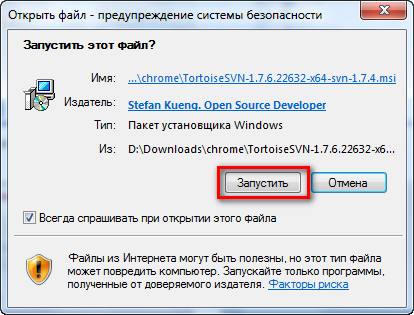
\includegraphics[scale=0.50]{tortoisesvn-instalation-step-2.png}
			\vspace{-10pt}
			\caption{Шаг 1}
		}
	\end{minipage}
	\begin{minipage}[h]{0.49\linewidth} 
		\center{
			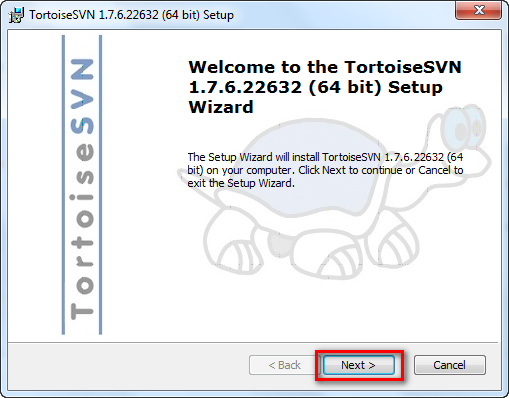
\includegraphics[scale=0.50]{tortoisesvn-instalation-step-3.png}
			\vspace{-10pt}
			\caption{Шаг 2}
		}
	\end{minipage}
\end{figure}

\vspace{-20pt}
 	
\begin{figure}[h!]
	\begin{minipage}[h]{0.49\linewidth}
		\center{
			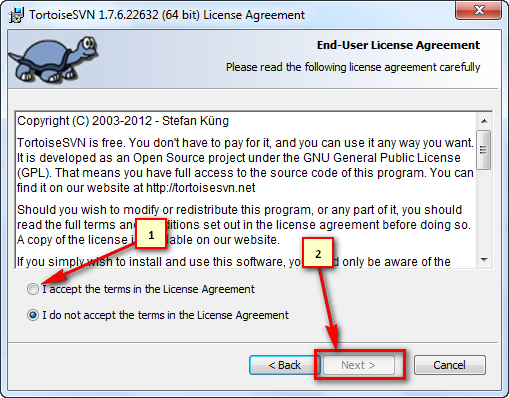
\includegraphics[scale=0.55]{tortoisesvn-instalation-step-4.png}
			\vspace{-10pt}
			\caption{Шаг 3}
		}
	\end{minipage}
	\hfill
	\begin{minipage}[h]{0.49\linewidth}
		\center{
			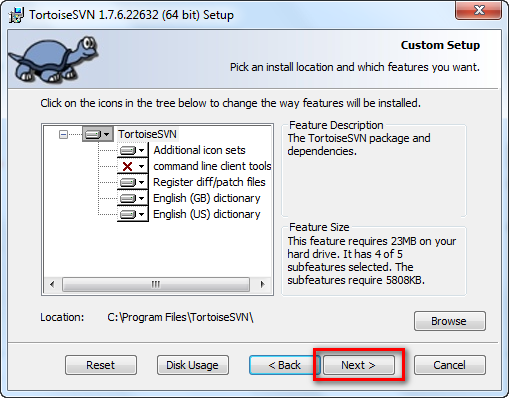
\includegraphics[scale=0.55]{tortoisesvn-instalation-step-5.png}
			\vspace{-10pt}
			\caption{м 4}
		}
	\end{minipage}
\end{figure}
\vspace{-20pt}

\begin{figure}[h!]
	\begin{minipage}[h]{0.49\linewidth}
		\center{
			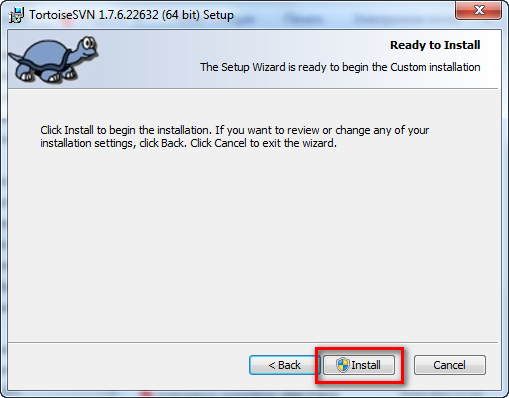
\includegraphics[scale=0.55]{tortoisesvn-instalation-step-6.png}
			\vspace{-10pt}
			\caption{Шаг 5}
		}
	\end{minipage}
	\hfill
	\begin{minipage}[h]{0.49\linewidth}
		\center{
			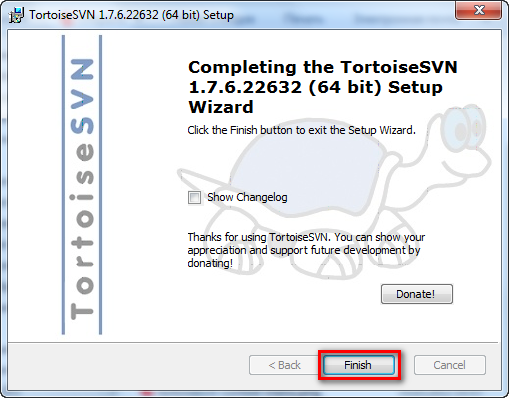
\includegraphics[scale=0.55]{tortoisesvn-instalation-step-7.png}
			\vspace{-10pt}
			\caption{Шаг 6}
		}
	\end{minipage}
\end{figure}

\subsubsection{Описание возможностей}

Для работы с TortoiseSVN используется интеграция с Проводником Windows
(Windows Explorer).

Для того чтобы выкачать проект из репозитория можно использовать диалог
``Checkout'' из меню проводника

\begin{figure}[h!]
	\begin{minipage}[h]{0.24\linewidth}
		\center{
			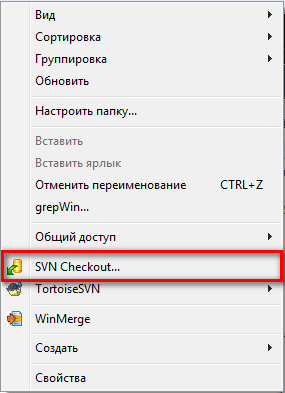
\includegraphics[scale=0.60]{tortoisesvn-work-instractions-step-1.png}
			\vspace{-10pt}
			\caption{Контекстное меню Проводника}
		}
	\end{minipage}
	\hfill
	\begin{minipage}[h]{0.75\linewidth}
		\center{
			\vspace{-25pt}
			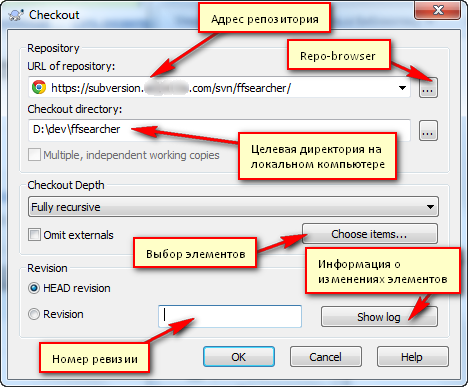
\includegraphics[scale=0.80]{tortoisesvn-work-instractions-step-2.png}
			\vspace{-10pt}
			\caption{Описание диалога ``Checkout''}
		}
	\end{minipage}
\end{figure}

После завершения процесса загрузки проекта появится диалог ``Checkout
Finished!''

\begin{figure}[h!]
	\centering
	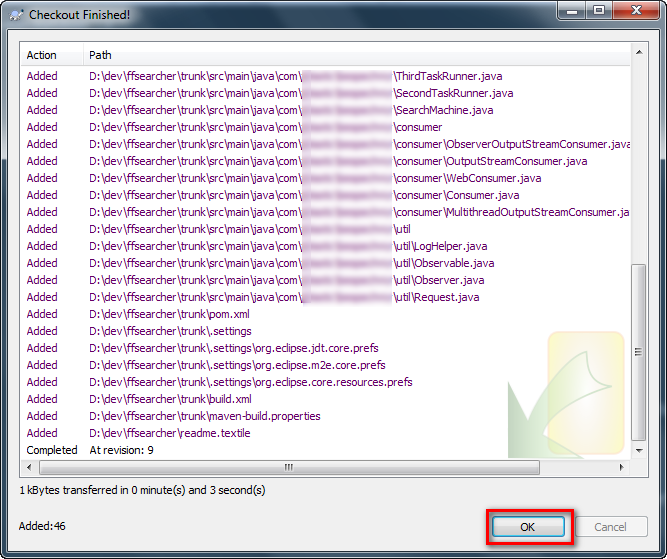
\includegraphics[scale=0.75]{tortoisesvn-work-instractions-step-3.png}
	\vspace{-10pt}
	\caption{Диалог ``Checkout Finished!''}
\end{figure}

В результате работы TortoiseSVN в релевой директории будет размещена
рабочая копия.

После изменения файлов для фиксации изменений можно воспользоваться
пунктом меню SVN Commit
\begin{figure}[h!]
	\centering
	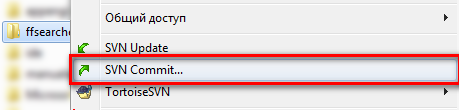
\includegraphics[scale=0.80]{tortoisesvn-work-instractions-step-4.png}
	\vspace{-10pt}
	\caption{Пункт меню SVN Commit}
\end{figure}
	
Далее вызывается диалог ``Commit''

\begin{figure}[h!]
	\centering
	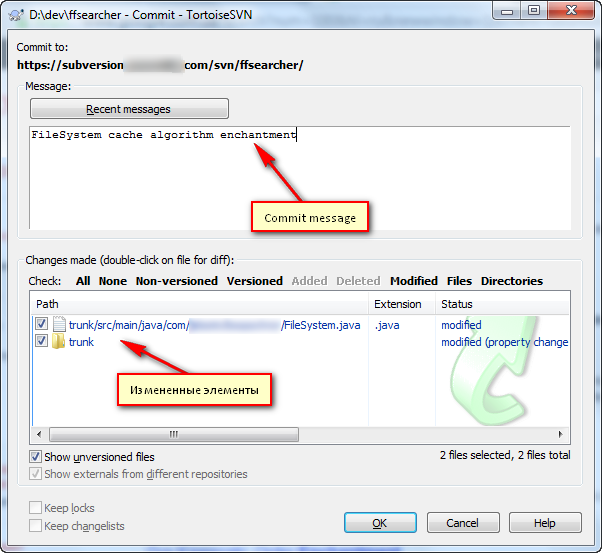
\includegraphics[scale=0.70]{tortoisesvn-work-instractions-step-5.png}
	\vspace{-10pt}
	\caption{Диалог ``Commit''}
\end{figure}

После завершения процесса фиксации показывается диалог ``Commit
Finished!''

\begin{figure}[h!]
	\centering
	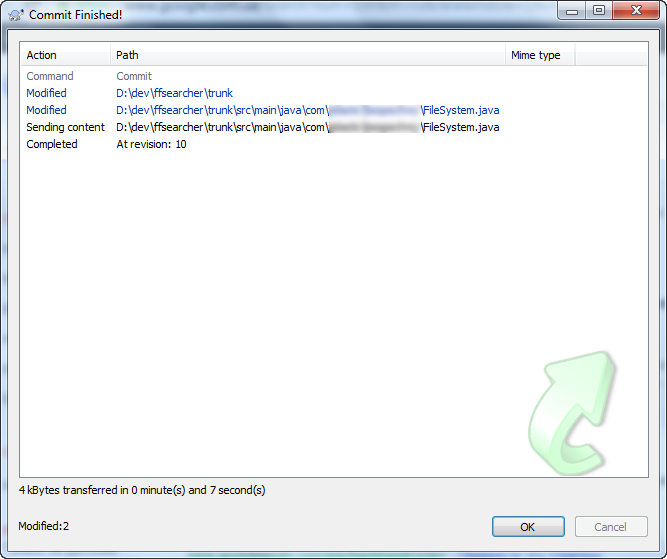
\includegraphics[scale=0.55]{tortoisesvn-work-instractions-step-6.png}
	\vspace{-10pt}
	\caption{Диалог ``Commit Finished!''}
\end{figure}

Для обновления рабочей копии можно использовать пункт меню ``SVN
Update''.

\begin{figure}[h!]
	\centering
	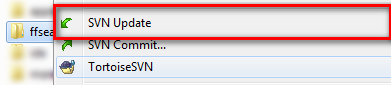
\includegraphics[scale=0.60]{tortoisesvn-work-instractions-step-7.png}
	\vspace{-10pt}
	\caption{Пункт меню ``SVN Update''}
\end{figure}

После обновления появится диалог ``Update Finished!''.

\begin{figure}[h!]
	\centering
	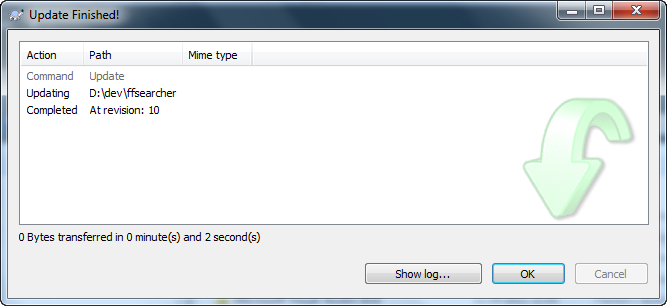
\includegraphics[scale=0.60]{tortoisesvn-work-instractions-step-8.png}
	\vspace{-10pt}
	\caption{Диалог ``Update Finished!''}
\end{figure}

\clearpage

\section{Интеграция с IDE}

Обычно для работы с системами контроля версий используется интеграция с
IDE. Для всех популярных IDE существуют плагины или функциональность
связанная с системами контроля версий есть в IDE из коробки.

\subsection{\href{http://www.jetbrains.com/idea/}{IntelliJ IDEA}}
\setcounter{figure}{0}
Интеграция с SVN в IDE IntelliJ IDEA присутствует out-of-the-box. Для
выкачивания проекта из репозитория используется диалог ``Checkout from
Subversion''. Его можно вызвать из меню
\texttt{VCS -\textgreater{} Checkout from Version Control -\textgreater{} Subversion}

\begin{figure}[h!]
	\centering
	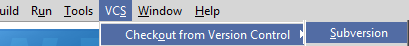
\includegraphics[scale=0.80]{intellij-idea-1.png}
	\vspace{-10pt}
	\caption{Меню для работы с Subversion}
\end{figure}
\vspace{-10pt}
В диалоге ``Checkout from Subversion'' можно добавить новый репозиторий. Это
можно сделать нажав кновку

\includegraphics[scale=0.80]{intellij-idea-add-repo.png}. В появившемся окне
необходимо ввести путь к репозиторию.

\begin{figure}[h!]
	\begin{minipage}[h]{0.49\linewidth}
		\center{
			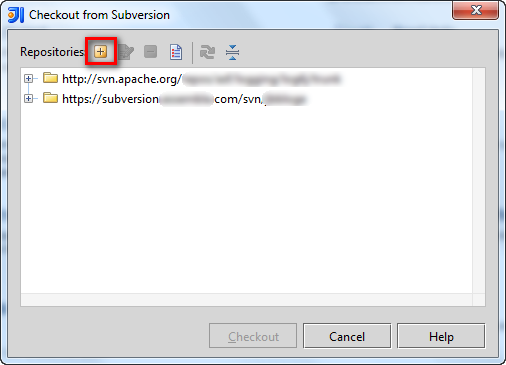
\includegraphics[scale=0.65]{intellij-idea-2.png}
			\vspace{-10pt}
			\caption{Диалог ``Checkout from Subversion''}
		}
	\end{minipage}
	\hfill
	\begin{minipage}[h]{0.49\linewidth}
		\center{
			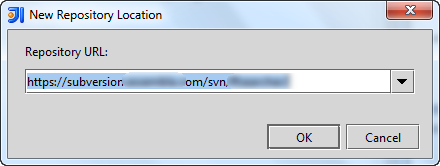
\includegraphics[scale=0.60]{intellij-idea-3.png}
			\vspace{-10pt}
			\caption{Ввод пути к репозиторию}
		}
	\end{minipage}
\end{figure}
 
Делее необходимо выбрать нужный репозиторий и нажать ``Checkout'' и выбрать
директорию, в которую будет помещена рабочая копия.
\begin{figure}[h!]
	\begin{minipage}[h]{0.49\linewidth}
		\center{
			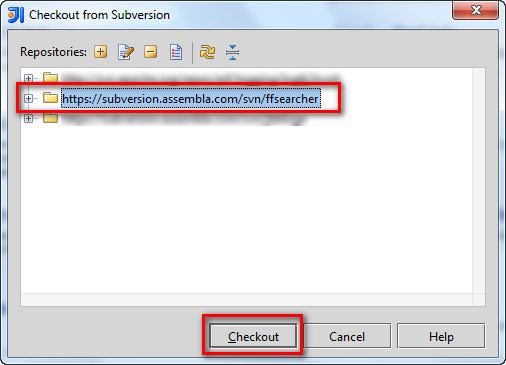
\includegraphics[scale=0.60]{intellij-idea-4.png}
			\vspace{-10pt}
			\caption{Диалог ``Checkout from Subversion''}
		}
	\end{minipage}
	\hfill
	\begin{minipage}[h]{0.49\linewidth}
		\center{
			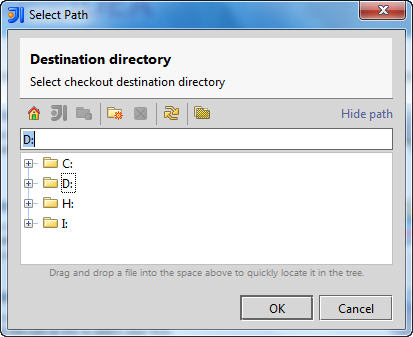
\includegraphics[scale=0.50]{intellij-idea-5.png}
			\vspace{-10pt}
			\caption{Выбор директории, в которую будет помещена рабочая копия}
		}
	\end{minipage}
\end{figure}

После этого появляется диалог ``SVN Checkout Options'', в котором есть
возможность выбрать ревизию. После нажатия на кнопку ``OK'' появится диалог
выбора формата (версии) рабочей копии.

\begin{figure}[h!]
	\begin{minipage}[h]{0.49\linewidth}
		\center{
			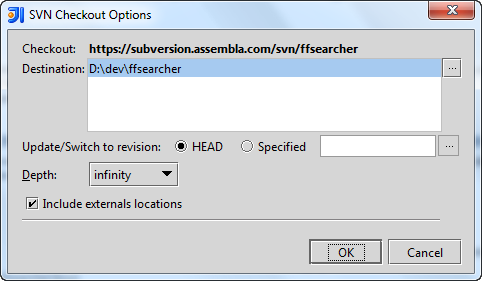
\includegraphics[scale=0.65]{intellij-idea-6.png}
			\vspace{-10pt}
			\caption{Диалог ``SVN Checkout Options''}
		}
	\end{minipage}
	\hfill
	\begin{minipage}[h]{0.49\linewidth}
		\center{
			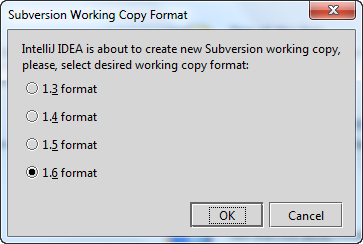
\includegraphics[scale=0.70]{intellij-idea-7.png}
			\vspace{-10pt}
			\caption{Выбор формата рабочей копии}
		}
	\end{minipage}
\end{figure}

Далее IntelliJ IDEA предложит создать проект из рабочей копии и, если была
нажата кнопка ``Yes'', выведется стандартный диалог создания нового проекта.

\begin{figure}[h!]
	\centering
	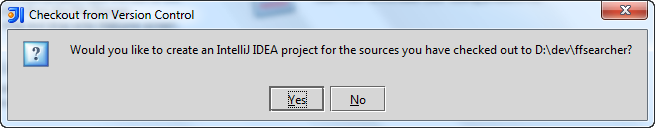
\includegraphics[scale=0.60]{intellij-idea-8.png}
	\vspace{-10pt}
	\caption{Диалог создания нового проекта}
\end{figure}
\vspace{-10pt}
\begin{figure}[h!]
	\centering
	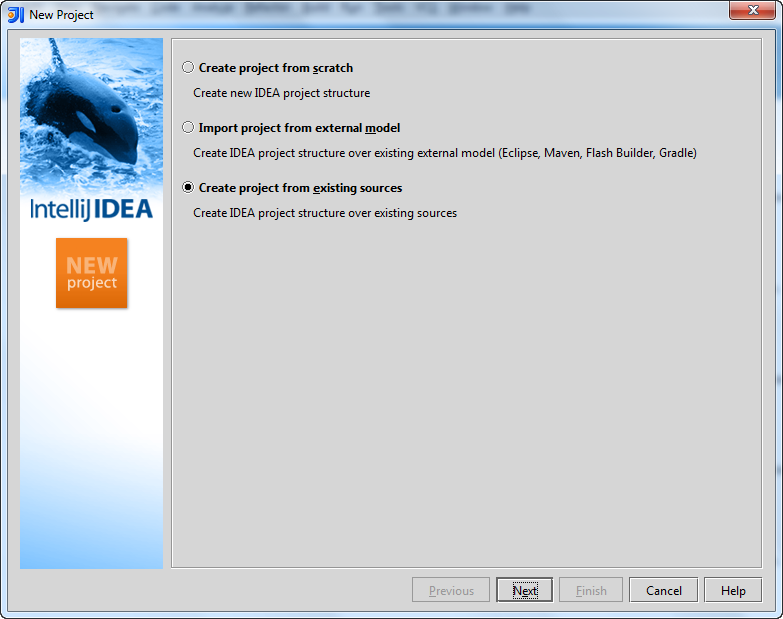
\includegraphics[scale=0.59]{intellij-idea-9.png}
	\vspace{-10pt}
	\caption{Диалог создания нового проекта}
\end{figure}

Для фиксации изменений можно использовать панель ``Changes''. На данной панели
расположены файлы, измененные после последней фиксации. Эту панель можно вызвать
комбинацией клавиш ``\texttt{Alt + 9}''. ``Default'' --- это список изменений.
По умолчанию в него добавляются все файлы, которые изменились в данном проекте, но
не были зафиксированы. 

\begin{figure}[h!]
	\centering
	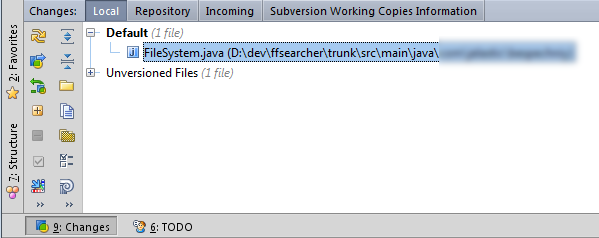
\includegraphics[scale=0.60]{intellij-idea-14.png}
	\vspace{-10pt}
	\caption{Панель управления изменениями}
\end{figure}

Для фиксации или отката изменений используется контекстное меню, которое можно
вызвать как у отдельного файла, так и списка изменений.

При выборе пункта меню ``Revert'' выводится диалог ``Revert Changes''. Данную
операцию можно применить к отдельным файлам и к спискам изменений.
\begin{figure}[h!]
	\begin{minipage}[h]{0.49\linewidth}
		\center{
			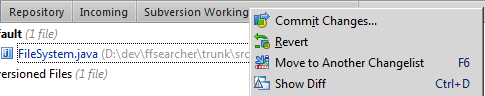
\includegraphics[scale=0.60]{intellij-idea-15.png}
			\vspace{-10pt}
			\caption{Контекстное меню панели управления	изменениями}
		}
	\end{minipage}
	\hfill
	\begin{minipage}[h]{0.49\linewidth}
		\center{
			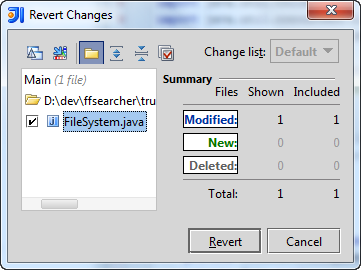
\includegraphics[scale=0.60]{intellij-idea-16.png}
			\vspace{-10pt}
			\caption{Откат изменений}
		}
	\end{minipage}
\end{figure}

При выборе пункта меню ``Commit Changes\ldots'' выводится диалог `Commit 
Changes''.
Данную операцию можно применить к отдельным файлам и к спискам изменений.

\begin{figure}[h!]
	\centering
	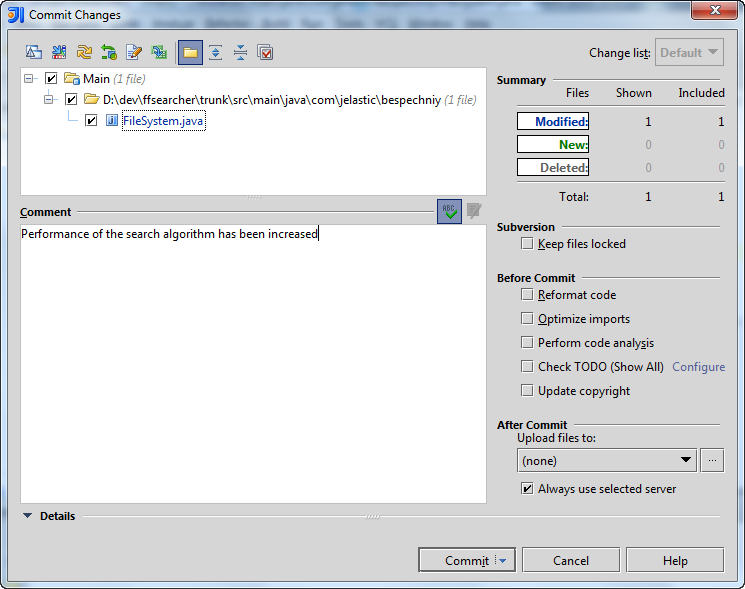
\includegraphics[scale=0.60]{intellij-idea-17.png}
	\vspace{-10pt}
	\caption{Фиксация изменений}
\end{figure}
Данный диалог имеет множество опций для контроля качества изменений.

\subsection{\href{http://www.eclipse.org/}{Eclipse}}
\setcounter{figure}{0}
Для платформы Eclipse доступно множество плагинов для работы с
систеами котроля версий.
\subsubsection{Установка необходимых плагинов}

Для SVN существует несколько популярных и активно развивающихся плагинов. Далее
будет рассмотрена установка и работа с плагином ``\texttt{Subversive - SVN Team
Provider}''. В данный момент это второй по популярности плагин, но он имеет ряд
достоинств перед лидером.

\paragraph{Установка плагина \texttt{Subversive} для Eclipse.}
Для установки плагинов удобно использовать \texttt{Eclipse Marketplace}. Клиент
можно вызвать использую меню \texttt{Help -\textgreater{} Eclipse
Marketplace\ldots}. Если клиент не установлен, ниже описан процесс его
установки.

\begin{figure}[h!]
	\centering
	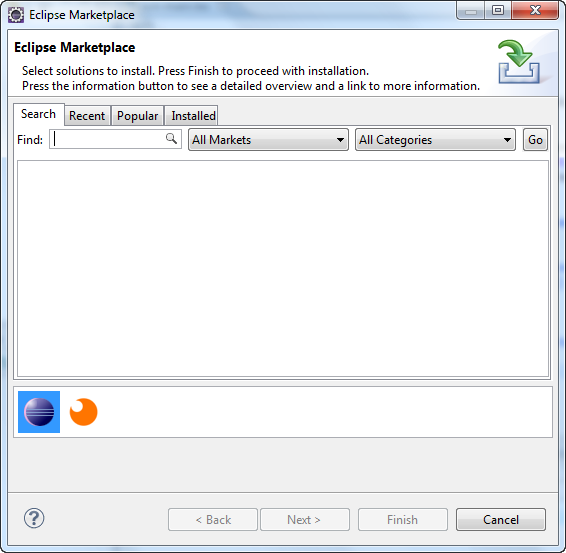
\includegraphics[scale=0.60]{eclipse-marketplace-instalation.png}
	\vspace{-10pt}
	\caption{Eclipse Marketplace}
\end{figure}

Для установки плагина в поле с меткой ``Find'' нужно ввести
``\texttt{Subversive}'' и выполнить поиск. После загрузки результатов поиска
нужно нажать на кнопку ``\texttt{Install}'' нужного плагина.

\paragraph{Установка клиента Eclipse Marketplace.}

Для установки клиента ``\texttt{Eclipse Marketplace}'' нужно вызвать диалог
``Install'' с помощью меню \texttt{Help -\textgreater{} Install New
Software\ldots} и в комбинированном списоке с меткой \texttt{Work with:} выбрать
``\texttt{Indigo}''.

В появившемся списке необходимо в списке ``\texttt{General Purpose Tools}''
отметить ``\texttt{Marketplace Client}'' и нажать на кнопку ``\texttt{Next}''.
\begin{figure}[h!]
	\centering
	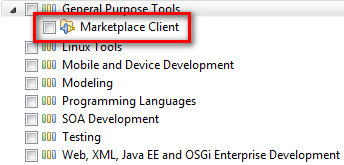
\includegraphics[scale=0.70]{eclipse-marketplace-instalation-1.png}
	\vspace{-10pt}
	\caption{Установка Eclipse Marketplace}
\end{figure}
Далее нужно следовать инструкциям по установке.

После установки в меню Help появится подменю Eclipse Marketplace\ldots.

\begin{figure}[h!]
	\centering
	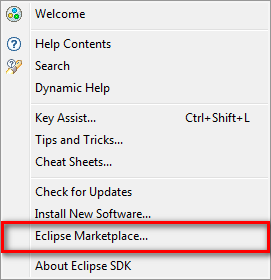
\includegraphics[scale=0.60]{eclipse-marketplace-instalation-7.png}
	\vspace{-10pt}
	\caption{Подменю Eclipse Marketplace}
\end{figure}

\subsubsection{Работа с SVN}

Для начала нужно открыть ``Package Explorer''. Это можно сделать
комбинацией клавиш ``Alt + Shift + Q, P'' или ``Window'' -\textgreater{}
``Show View'' -\textgreater{} ``Package Explorer''.

\begin{figure}[h!]
	\centering
	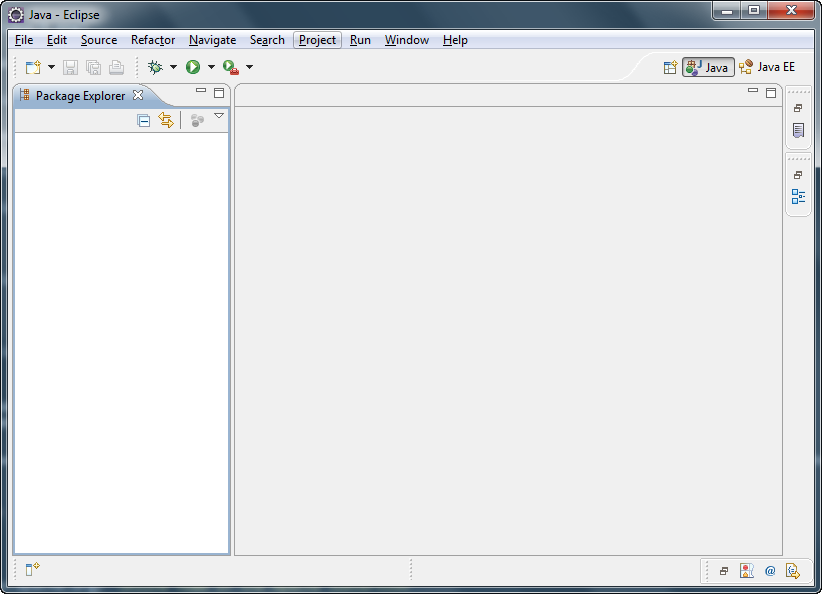
\includegraphics[scale=0.60]{eclipse.png}
	\caption{Package Explorer}
\end{figure}

Далее выполняем File -\textgreater{} Import или:

\begin{figure}[h!]
	\centering
	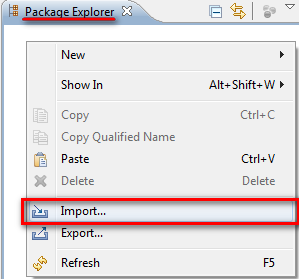
\includegraphics[scale=0.60]{eclipse-checkout-step-1.png}
	\caption{Импорт проекта}
\end{figure}

После этого появится диалог ``Import''. В этом диалоге находится список
всех поддерживаемых Вашей сборкой Eclipse типов проектов. Необходимо
выбрать из этого списка SVN -\textgreater{} Project from SVN и нажать на
кнопку Next.

\begin{figure}[h!]
	\centering
	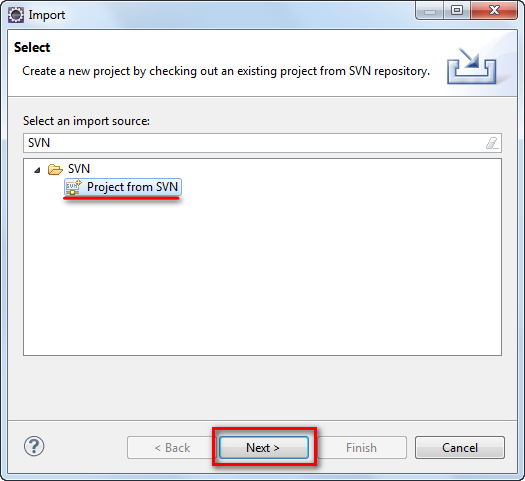
\includegraphics[scale=0.80]{eclipse-checkout-step-2.png}
	\vspace{-10pt}
	\caption{Диалог ``Import''}
\end{figure}

На следующем шаге Вы должны выбрать одну из существующих записей о
репозиториях или же создать новую. На данном шаге нужно выбрать ``Create
a new repository location'' и нажать на кнопку Next.

\begin{figure}[h!]
	\centering
	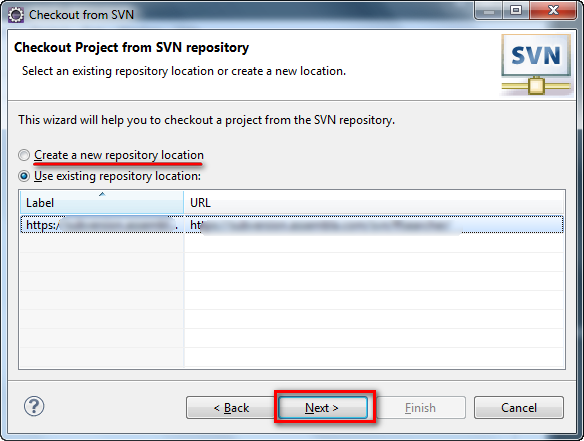
\includegraphics[scale=0.80]{eclipse-checkout-step-3.png}
	\vspace{-10pt}
	\caption{Диалог ``Checkout form SVN''}
\end{figure}

Следующий шаг заключается в заполнении нескольких полей. Если
репозиторий, который Вы указали в поле URL требует автризации, Вам также
необходимо будет заполнить поля User и Password. Если Вы не хотите чтобы
Eclipse постоянно просил ввести login и password для доступа к
репоситорию отметьте ``Save authentication'' и нажмите на кнопку Next.

\begin{figure}[h!]
	\centering
	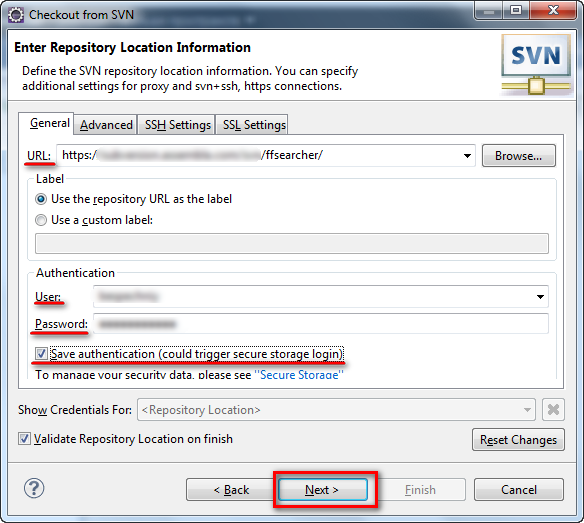
\includegraphics[scale=0.80]{eclipse-checkout-step-4.png}
	\vspace{-10pt}
	\caption{Диалог ``Checkout form SVN''}
\end{figure}

На следующем шаге необходимо ввести название ветки, которая будет
импортирована как проект. В данном случае checkout будет выполнен из
trunk. Также в данном диалоге можно выбрать ревизию (HEAD в случаем если
из репозитория нужно забрать последнюю версию исходных кодов).

\begin{figure}[h!]
 	\centering
	\includegraphics[scale=0.80]{eclipse-checkout-step-5.png}
	\vspace{-10pt}
	\caption{Диалог ``Checkout form SVN''}
\end{figure}

Далее Eclipse проведет анализ проекта и выведет диалог в котором
предложет ввести имя проекта для которого будет выполнен checkout, а
также значение Depth и ревизию.

\begin{figure}[h!]
	\centering
	\includegraphics[scale=1]{eclipse-checkout-step-6.png}
	\vspace{-10pt}
	\caption{Диалог ``Check Out As''}
\end{figure}

После нажатия на кнопку Finish, Eclipse выкачает проект и отобразит его
в Package Explorer.

\begin{figure}[h!]
	\centering
	\includegraphics[scale=1]{eclipse-2.png}
	\vspace{-10pt}
	\caption{Вид ``Package Explorer''}
\end{figure}

В Package Eplorer также можно увидеть ревизию, в которой изменялся тот
или иной файл.

Внесем изменения. После сохранения измененного файла в Package Explorer
можно увидеть символ ``\textgreater{}'' около него.

\begin{figure}[h!]
	\centering
	\includegraphics[scale=0.90]{eclipse-3.png}
	\vspace{-10pt}
	\caption{Вид ``Package Explorer''}
\end{figure}

Перед выполнением фиксации изменений обычно сравнивают BASE версию и
текущую версию, чтобы просмотреть изменения которые должны попасть в
репозиторий. Чтобы просмотреть изменения в проекте кликните ПКМ на
проекте в Package Explorer и далее Compare With -\textgreater{} Base
from Working Copy.

\begin{figure}[h!]
	\centering
	\includegraphics[scale=0.80]{eclipse-diff-1.png}
	\vspace{-10pt}
	\caption{Меню просмотра изменений}
\end{figure}

В данном случае в проекте только одно изменение.
\begin{figure}[h!]
	\centering
	\includegraphics[scale=0.80]{eclipse-diff-2.png}
	\vspace{-10pt}
	\caption{Просмотр изменений}
\end{figure}

Как видно из сравнения, изменение заключается в добавлении модификатора
volatile в объявлении поля класса.

Далее выполним фиксацию изменений. Для этого можно использовать
комбинацию клавиш ``Ctrl + Alt + C'' или в Package Explorer кликнуть ПКМ
на проекте и далее ``Team -\textgreater{} Commit\ldots{}''.

\begin{figure}[h!]
	\centering
	\includegraphics[scale=0.60]{eclipse-commit-1.png} 
	\vspace{-10pt}
	\caption{Меню Team}
\end{figure}

В диалоге ``Commit''
необходимо ввести Commit message. Также в списке можно увидеть
измененные файлы. Файлы которые должны попать в репозиторий под данным
коммитом нужно отметить (по умолчанию отмечены все).

\begin{figure}[h!]
	\centering
	\includegraphics[scale=0.60]{eclipse-commit-2.png} 
	\vspace{-10pt}
	\caption{Диалог Commit}
\end{figure}
После нажатия на кнопку Ok все изменения будут отправлены в репозиторий. 
Также в Package Explorer поменяется ревизия всех зафиксированных файлов.

Для выполнения обновления проекта можно использовать комбинацию клавиш
Ctrl + Alt + U или в Package Explorer кликнуть ПКМ на проекте и далее
``Team -\textgreater{} Update''.

\begin{figure}[h!]
	\centering
	\includegraphics[scale=0.80]{eclipse-update-1.png}
	\vspace{-10pt}
	\caption{Обновление проекта}
\end{figure}

\subsection{\href{http://netbeans.org/}{NetBeans}}
\setcounter{figure}{0}
Для выполнения checkout используется меню ``Группа -\textgreater{}
Система управления исходным кодом Subversion -\textgreater{} Получить''.

\begin{figure}[h!]
	\centering
	\includegraphics[scale=0.90]{netbeans-checkout-1.png}
	\vspace{-10pt}
	\caption{Меню ``Группа''}
\end{figure}

Далее появляется диалог ``Получение'' в котором необходимо ввести URL к
репозиторию (если этот репозиторий требует авторизацию, то дополнительно
нужно заполнить поля ``Пользователь'' и ``Пароль'').

\begin{figure}[h!]
	\centering
	\includegraphics[scale=0.90]{netbeans-checkout-2.png}
	\vspace{-10pt}
	\caption{Диалог ``Получение''}
\end{figure}

После клика на кнопку ``Далее'', NetBeans предлагает ввести директорию,
из которой будут выкачаны исходные тексты. Также на форме можно выбрать
ревизию (по умолчанию HEAD) и директорию в которую будет сохранена
рабочая копия.

\begin{figure}[h!]
	\centering
	\includegraphics[scale=0.90]{netbeans-checkout-3.png}
	\vspace{-10pt}
	\caption{Диалог ``Получение''}
\end{figure}

После завершения работы мастера NetBeans выкачает исходные коды и
предложит открыть их как проект.

\begin{figure}[h!]
	\centering
	\includegraphics[scale=0.80]{netbeans-checkout-4.png}
	\vspace{-10pt}
	\caption{Диалог ``Получение завершено''}
\end{figure}

После открытия в dock ``Проекты'' должен появиться новый проект.

\begin{figure}[h!]
	\centering
	\includegraphics[scale=0.85]{netbeans-1.png}
	\caption{Боковая панель ``Проекты''}
\end{figure}

Внесем изменения. После сохранения измененного файла dock ``Проекты'' он
будет подсвечен.

\begin{figure}[h!]
	\centering
	\includegraphics[scale=0.85]{netbeans-2.png}
	\caption{Боковая панель ``Проекты'' с подсвеченным файлом}
\end{figure}

Для просмотра изменений надо нажать ПКМ на проекте или на конкретном
файле, и далее ``Система управления исходным кодом Subversion
-\textgreater{} Различия''. 

\begin{figure}[h!]
	\centering
	\includegraphics[scale=0.90]{netbeans-diff-1.png}
	\caption{Контекстное меню боковой панели ``Проекты''}
\end{figure}

Далее открывается вкладка ``Различия'', на которой видно, что текущее
изменение заключалось в замене примитива синхронизации Semaphore на
Lock, а конкретно на ReentrantLock.

\begin{figure}[h!]
	\centering
	\includegraphics[scale=0.80]{netbeans-diff-2.png}
	\caption{Просмотр изменений}
\end{figure}

После проверки, и отмены всех не нужных изменений в файле, который нужно
отправить в репозиторий, можно выполнить фиксацию.

Для фиксации изменений необходимо кликнуть ПКМ на проекте или файле,
далее ``Система управления исходным кодом Subversion -\textgreater{}
Фиксация\ldots{}''.

\begin{figure}[h!]
	\centering
	\includegraphics[scale=0.70]{netbeans-commit-1.png}
	\caption{Меню ``Система управления исходным кодом Subversion''}
\end{figure}

В появившемся окне нужно ввести комментарий к фиксации, и выбрать файлы,
для отправки в репозиторий.

\begin{figure}[h!]
	\centering
	\includegraphics[scale=0.70]{netbeans-commit-2.png}
	\caption{Диалог ``Фиксация''}
\end{figure}

После нажатия на кнопку ``Фиксировать'' NetBeans отправит изменения в
репозиторий.

Для обновления проекта необходимо кликнуть ПКМ на проекте, далее
``Система управления исходным кодом Subversion -\textgreater{}
Обновить''.

\begin{figure}[h!]
\centering
\includegraphics[scale=0.60]{netbeans-update-1.png}
\caption{Обновление}
\end{figure}

Далее NetBeans выполнит обновление проекта к HEAD ревизиий.

\end{document}